\documentclass{standalone}
\usepackage{tikz}
\usetikzlibrary{patterns, positioning}


\begin{document}
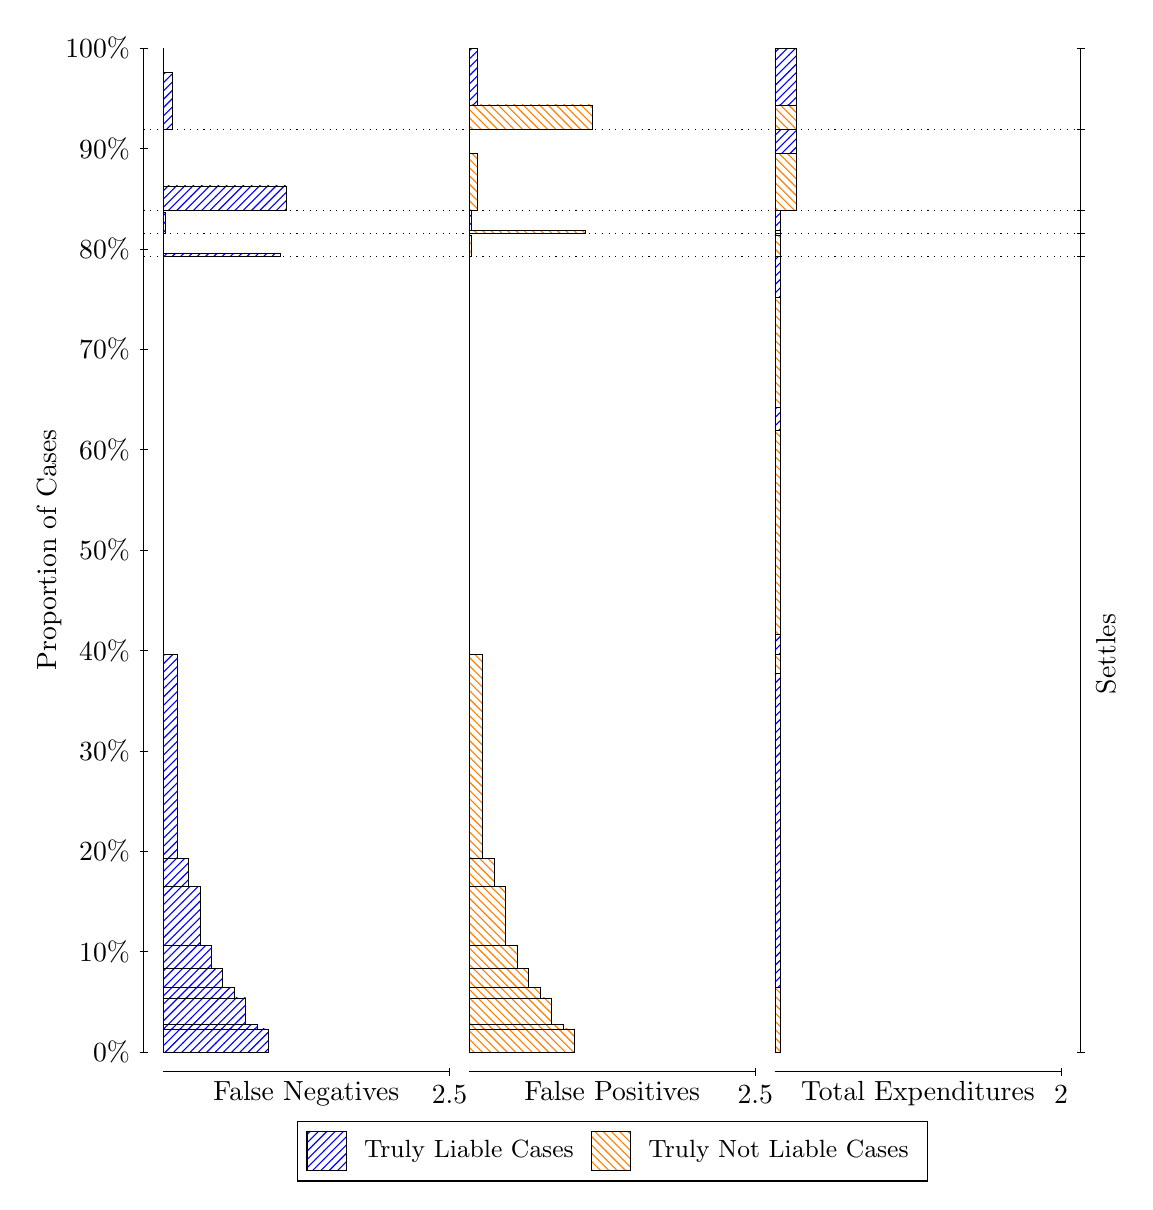
\begin{tikzpicture}
\draw[black, very thin] (1.5,1.75) -- (1.5,14.5);
\node[rotate=90, text=black, anchor=center] at (0.3, 8.125) {Proportion of Cases};
\draw[black, very thin] (1.45,1.75) -- (1.55,1.75);
\node[text=black, anchor=east] at (1.45, 1.75) {0\%};
\draw[black, very thin] (1.45,3.025) -- (1.55,3.025);
\node[text=black, anchor=east] at (1.45, 3.025) {10\%};
\draw[black, very thin] (1.45,4.3) -- (1.55,4.3);
\node[text=black, anchor=east] at (1.45, 4.3) {20\%};
\draw[black, very thin] (1.45,5.575) -- (1.55,5.575);
\node[text=black, anchor=east] at (1.45, 5.575) {30\%};
\draw[black, very thin] (1.45,6.85) -- (1.55,6.85);
\node[text=black, anchor=east] at (1.45, 6.85) {40\%};
\draw[black, very thin] (1.45,8.125) -- (1.55,8.125);
\node[text=black, anchor=east] at (1.45, 8.125) {50\%};
\draw[black, very thin] (1.45,9.4) -- (1.55,9.4);
\node[text=black, anchor=east] at (1.45, 9.4) {60\%};
\draw[black, very thin] (1.45,10.675) -- (1.55,10.675);
\node[text=black, anchor=east] at (1.45, 10.675) {70\%};
\draw[black, very thin] (1.45,11.95) -- (1.55,11.95);
\node[text=black, anchor=east] at (1.45, 11.95) {80\%};
\draw[black, very thin] (1.45,13.225) -- (1.55,13.225);
\node[text=black, anchor=east] at (1.45, 13.225) {90\%};
\draw[black, very thin] (1.45,14.5) -- (1.55,14.5);
\node[text=black, anchor=east] at (1.45, 14.5) {100\%};

\draw[black, very thin] (13.4,1.75) -- (13.4,14.5);
\draw[black, very thin] (13.35,1.75) -- (13.45,1.75);
\node[anchor=west] at (13.35, 1.75) {};
\draw[black, very thin] (13.35,11.858) -- (13.45,11.858);
\node[anchor=west] at (13.35, 11.858) {};
\draw[black, very thin] (13.35,12.15) -- (13.45,12.15);
\node[anchor=west] at (13.35, 12.15) {};
\draw[black, very thin] (13.35,12.442) -- (13.45,12.442);
\node[anchor=west] at (13.35, 12.442) {};
\draw[black, very thin] (13.35,13.471) -- (13.45,13.471);
\node[anchor=west] at (13.35, 13.471) {};
\draw[black, very thin] (13.35,14.5) -- (13.45,14.5);
\node[anchor=west] at (13.35, 14.5) {};

\draw[black, very thin, pattern color=blue, pattern=north east lines] (1.75,1.75) rectangle (3.0852,2.042);
\draw[black, very thin, pattern color=blue, pattern=north east lines] (1.75,2.042) rectangle (2.9399,2.0996);
\draw[black, very thin, pattern color=blue, pattern=north east lines] (1.75,2.0996) rectangle (2.7946,2.4358);
\draw[black, very thin, pattern color=blue, pattern=north east lines] (1.75,2.4358) rectangle (2.6492,2.5656);
\draw[black, very thin, pattern color=blue, pattern=north east lines] (1.75,2.5656) rectangle (2.5039,2.8145);
\draw[black, very thin, pattern color=blue, pattern=north east lines] (1.75,2.8145) rectangle (2.3586,3.1065);
\draw[black, very thin, pattern color=blue, pattern=north east lines] (1.75,3.1065) rectangle (2.2133,3.855);
\draw[black, very thin, pattern color=blue, pattern=north east lines] (1.75,3.855) rectangle (2.0679,4.2076);
\draw[black, very thin, pattern color=blue, pattern=north east lines] (1.75,4.2076) rectangle (1.9226,6.8038);
\draw[black, very thin, pattern color=orange, pattern=north west lines] (1.75,6.8038) rectangle (1.75,11.858);
\draw[black, very thin, pattern color=blue, pattern=north east lines] (1.75,11.858) rectangle (3.2306,11.89);
\draw[black, very thin, pattern color=orange, pattern=north west lines] (1.75,11.89) rectangle (1.75,12.15);
\draw[black, very thin, pattern color=blue, pattern=north east lines] (1.75,12.15) rectangle (1.7773,12.41);
\draw[black, very thin, pattern color=orange, pattern=north west lines] (1.75,12.41) rectangle (1.75,12.442);
\draw[black, very thin, pattern color=blue, pattern=north east lines] (1.75,12.442) rectangle (3.3123,12.749);
\draw[black, very thin, pattern color=orange, pattern=north west lines] (1.75,12.749) rectangle (1.75,13.471);
\draw[black, very thin, pattern color=blue, pattern=north east lines] (1.75,13.471) rectangle (1.859,14.193);
\draw[black, very thin, pattern color=orange, pattern=north west lines] (1.75,14.193) rectangle (1.75,14.5);
\draw[black, very thin, pattern color=orange, pattern=north west lines] (5.6333,1.75) rectangle (6.9686,2.042);
\draw[black, very thin, pattern color=orange, pattern=north west lines] (5.6333,2.042) rectangle (6.8233,2.0996);
\draw[black, very thin, pattern color=orange, pattern=north west lines] (5.6333,2.0996) rectangle (6.6779,2.4357);
\draw[black, very thin, pattern color=orange, pattern=north west lines] (5.6333,2.4357) rectangle (6.5326,2.5656);
\draw[black, very thin, pattern color=orange, pattern=north west lines] (5.6333,2.5656) rectangle (6.3873,2.8145);
\draw[black, very thin, pattern color=orange, pattern=north west lines] (5.6333,2.8145) rectangle (6.2419,3.1065);
\draw[black, very thin, pattern color=orange, pattern=north west lines] (5.6333,3.1065) rectangle (6.0966,3.855);
\draw[black, very thin, pattern color=orange, pattern=north west lines] (5.6333,3.855) rectangle (5.9513,4.2076);
\draw[black, very thin, pattern color=orange, pattern=north west lines] (5.6333,4.2076) rectangle (5.8059,6.8039);
\draw[black, very thin, pattern color=blue, pattern=north east lines] (5.6333,6.8039) rectangle (5.6333,11.858);
\draw[black, very thin, pattern color=orange, pattern=north west lines] (5.6333,11.858) rectangle (5.6606,12.118);
\draw[black, very thin, pattern color=blue, pattern=north east lines] (5.6333,12.118) rectangle (5.6333,12.15);
\draw[black, very thin, pattern color=orange, pattern=north west lines] (5.6333,12.15) rectangle (7.1139,12.182);
\draw[black, very thin, pattern color=blue, pattern=north east lines] (5.6333,12.182) rectangle (5.6606,12.442);
\draw[black, very thin, pattern color=orange, pattern=north west lines] (5.6333,12.442) rectangle (5.7423,13.165);
\draw[black, very thin, pattern color=blue, pattern=north east lines] (5.6333,13.165) rectangle (5.6333,13.471);
\draw[black, very thin, pattern color=orange, pattern=north west lines] (5.6333,13.471) rectangle (7.1957,13.778);
\draw[black, very thin, pattern color=blue, pattern=north east lines] (5.6333,13.778) rectangle (5.7423,14.5);
\draw[black, very thin, pattern color=orange, pattern=north west lines] (9.5167,1.75) rectangle (9.5848,2.5656);
\draw[black, very thin, pattern color=blue, pattern=north east lines] (9.5167,2.5656) rectangle (9.5848,6.5549);
\draw[black, very thin, pattern color=orange, pattern=north west lines] (9.5167,6.5549) rectangle (9.5848,6.8038);
\draw[black, very thin, pattern color=blue, pattern=north east lines] (9.5167,6.8038) rectangle (9.5848,7.0527);
\draw[black, very thin, pattern color=orange, pattern=north west lines] (9.5167,7.0527) rectangle (9.5848,9.649);
\draw[black, very thin, pattern color=blue, pattern=north east lines] (9.5167,9.649) rectangle (9.5848,9.941);
\draw[black, very thin, pattern color=orange, pattern=north west lines] (9.5167,9.941) rectangle (9.5848,11.334);
\draw[black, very thin, pattern color=blue, pattern=north east lines] (9.5167,11.334) rectangle (9.5848,11.858);
\draw[black, very thin, pattern color=orange, pattern=north west lines] (9.5167,11.858) rectangle (9.5848,12.118);
\draw[black, very thin, pattern color=blue, pattern=north east lines] (9.5167,12.118) rectangle (9.5848,12.15);
\draw[black, very thin, pattern color=orange, pattern=north west lines] (9.5167,12.15) rectangle (9.5848,12.182);
\draw[black, very thin, pattern color=blue, pattern=north east lines] (9.5167,12.182) rectangle (9.5848,12.442);
\draw[black, very thin, pattern color=orange, pattern=north west lines] (9.5167,12.442) rectangle (9.7892,13.165);
\draw[black, very thin, pattern color=blue, pattern=north east lines] (9.5167,13.165) rectangle (9.7892,13.471);
\draw[black, very thin, pattern color=orange, pattern=north west lines] (9.5167,13.471) rectangle (9.7892,13.778);
\draw[black, very thin, pattern color=blue, pattern=north east lines] (9.5167,13.778) rectangle (9.7892,14.5);
\draw[black, dotted] (1.5,11.858) -- (13.4,11.858);
\draw[black, dotted] (1.5,12.15) -- (13.4,12.15);
\draw[black, dotted] (1.5,12.442) -- (13.4,12.442);
\draw[black, dotted] (1.5,13.471) -- (13.4,13.471);
\draw[black, very thin] (1.75,1.5) -- (5.3833,1.5);
\node[text=black, anchor=north] at (3.5667, 1.5) {False Negatives};
\draw[black, very thin] (5.3833,1.45) -- (5.3833,1.55);
\node[text=black, anchor=north] at (5.3833, 1.45) {2.5};

\draw[black, very thin] (5.6333,1.5) -- (9.2667,1.5);
\node[text=black, anchor=north] at (7.45, 1.5) {False Positives};
\draw[black, very thin] (9.2667,1.45) -- (9.2667,1.55);
\node[text=black, anchor=north] at (9.2667, 1.45) {2.5};

\draw[black, very thin] (9.5167,1.5) -- (13.15,1.5);
\node[text=black, anchor=north] at (11.333, 1.5) {Total Expenditures};
\draw[black, very thin] (13.15,1.45) -- (13.15,1.55);
\node[text=black, anchor=north] at (13.15, 1.45) {2};

\node[text=black, centered, rotate=90] at (13.72, 6.8039) {Settles};





\draw (7.449999999999999,1.5) node[draw=none] (baseCoordinate) {};
\begin{scope}[align=center]
        \matrix[scale=0.5, draw=black, below=0.5cm of baseCoordinate, nodes={draw}, column sep=0.1cm]{
            \node[rectangle, draw, minimum width=0.5cm, minimum height=0.5cm, pattern color=blue, pattern=north east lines] {}; &
            \node[draw=none, font=\small, text=black] (B) {Truly Liable Cases}; &
            \node[rectangle, draw, minimum width=0.5cm, minimum height=0.5cm, pattern color=orange, pattern=north west lines] {}; &
            \node[draw=none, font=\small, text=black] (B) {Truly Not Liable Cases}; \\
            };
\end{scope}

\end{tikzpicture}
\end{document}